\documentclass[sigconf]{acmart}
\settopmatter{printacmref=false} % Removes citation information below abstract
\renewcommand\footnotetextcopyrightpermission[1]{} % removes footnote with conference information in first column
\pagestyle{plain} % removes running headers
\setcopyright{none}

\usepackage{booktabs} % For formal tables
\usepackage[ruled]{algorithm2e} % For algorithms
\renewcommand{\algorithmcfname}{ALGORITHM}
\SetAlFnt{\small}
\SetAlCapFnt{\small}
\SetAlCapNameFnt{\small}
\SetAlCapHSkip{0pt}
\IncMargin{-\parindent}

\usepackage[latin1]{inputenc}
\usepackage{graphicx}
\usepackage{mathtools}
\usepackage{amsfonts}
\usepackage{multirow}

\DeclareMathOperator*{\argmax}{arg\,max\,}

\begin{document}

\title{Named Entity Recognition on HTML as a web data extraction subtask}

\author{João Mateus de Freitas Veneroso}
\affiliation{%
  \institution{Universidade Federal de Minas Gerais}
  \streetaddress{Av. Pres. Antônio Carlos, 6627 - Pampulha}
  \city{Belo Horizonte}
  \state{MG}
  \postcode{31270-901}
  \country{Brazil}}
\email{jmfveneroso@gmail.com}

\author{Berthier Ribeiro-Neto}
\affiliation{%
  \institution{Universidade Federal de Minas Gerais}
  \streetaddress{Av. Pres. Antônio Carlos, 6627 - Pampulha}
  \city{Belo Horizonte}
  \state{MG}
  \postcode{31270-901}
  \country{Brazil}}
\email{berthier.dcc.ufmg@gmail.com}

\begin{abstract}

Reliable researcher affiliation data is necessary to allow enquiring
about international research group productivity and publication patterns.
Public bibliographic databases such as DBLP and Google Scholar hold
invaluable data about the academic environment. However, the researcher
affiliation information is frequently missing or outdated.
We propose a statistical data extraction method to acquire affiliation 
information directly from university websites and solve the name extraction
task in general.
Previous approaches to web data extraction either lack in flexibility,
because wrappers do not generalize well on cross website tasks, or 
they lack in precision, because domain agnostic methods neglect 
useful properties of this particular application domain.
Our statistical approach solves the name extraction task with 
a framework that incorporates both textual and structural features to
yield an outstanding tradeoff between generality and precision. 
We conducted experiments over a collection of 152 faculty 
web pages in multiple languages from universities in 49 countries
and obtained 94.40\% precision, 97.61\% recall and 0.9597 F-measure at
the extraction task.


\end{abstract}

% \keywords{Named entity recognition, information extraction, web data extraction}

\maketitle

% ==========================================
% Beginning of text.                       |
% ==========================================

\section{Introduction}

Web data extraction (WDE) is the task of automatically extracting structured information
from unstructured or semi-structured web documents. The input usually consists of
web documents containing a number of predetermined entities organized in a similar 
manner and the information extraction task consists of identifying these entities
and organizing them according to a template. In this context, named entity recognition
(NER) is a subtask that aims to detect named entities in the text and classify them into 
predetermined categories such as person names, locations or organizations. 

HTML documents most often lie in between the structured / unstructured data paradigm.
DOM hierarchy, element disposition, class names, and other features related to 
the document structure and indirectly associated with the data itself can be valuable 
information in the task of identifying entities and determining relationships. Yet we 
cannot expect these features to be completely constrained by an underlying pattern. 
Organization patterns tend to follow some guidelines but are in no way subject to 
strict rules. That is why classical information extraction systems such as automatic
wrapper generators usually do not translate well across different websites. 

Most existing web data extraction methods are tailored to extract data from a single
web page \cite{Crescenzi2001, Arasu2003, Freitag1998, Califf1999, Soderland1999,
Kushmerick2000, Hsu1998, Muslea1999}, producing different compromises between efficacy
and degree of human supervision. More recent unsupervised approaches proposed to
tackle the problem of data extraction for whole application domains \cite{Zhu2005, Zhu2006, 
Abdessalem2010, Furche2012, Furche2012a}. Unsupervised WDE methods usually operate in at
least two steps: record segmentation and attribute labelling. Record segmentation
is essentially clustering visually and structurally similar web page regions and 
identifying repeating data records. Attribute labelling is the task of identifying
attributes in data records. Doing any of these tasks well can help performing the 
other task, since patterns that are present in some data records can help identifying 
attributes in other data records. And by properly identifying attributes, we are better 
able to determine the boundaries of data records and segment them with increased accuracy.

In recent years, we saw an astonishing progress in Natural Language Processing.
However, despite WDE being a closely related field of research,
many tools rely on heuristics or hand coded rules to perform record segmentation,
and many methods resort to regular expressions or gazetteer matching to perform attribute
labelling. While these approaches can be sufficient to extract information from webpages
with similar templates, and identifying attributes with distinct formats like prices and
dates, we still lack a sufficiently flexible and intelligent approach to handle more complicated cases.
Even when extracting data from web documents only, data records may contain pure text with 
relevant named entities. Also, many WDE algorithms can effectively exploit the semi-
structure of web documents, but when a method relies too much on structural features, it
often produces poor generalization on cross website extraction tasks. Contrastingly, we 
understand that statistical based approaches can be much more flexible.

In this paper, we investigate the attribute labelling task in WDE with a named entity 
recognition framework. Recently proposed neural architectures have achieved exciting results 
on the NER task on plain text \cite{Huang2015, Lample2016, Ma2016} while requiring almost 
no feature engineering or gazetteers. NER on HTML poses a different type of challenge, 
because web pages are often very different from plain text. Named entities may be present 
inside tables, lists, graphs or other types of visual elements that provide
little to no textual information that could give hints about the semantic category of 
a word. However we show that we can get exceptional performance even with this limitation
and small training sets.

By reliably detecting named entities, we can improve the performance of existing WDE 
approaches or even construct a full machine learning based tool to tackle domain wide
extraction with great flexibility. To test different NER approaches from the perspective 
of web data extraction,
we explored the task of person names extraction from university faculty listings.
Researcher affiliation is often missing from many entries in public databases 
and the display of information varies significantly between different university 
websites, so this task can provide a good measure of the expected performance and
data need for other web data extraction tasks. 

\section{Related Work}

In the last 20 years, the astonishing growth of public information in the web has 
led to the development of a number of different approaches to the problem of web 
information extraction. Traditionally, the task was solved by designing special purpose
programs called wrappers to recognize relevant data and store records in a structured
format. These early tools varied wildly relative to their degree of automation. 

It was readily perceived that manual wrapper generation was a rather tedious and
error prone process, unsuited for large scale operations. Wrappers tend to
break frequently because they rely heavily on web page features that can change 
often. So, in the late nineties, several authors advocated for wrapper induction, a technique 
that consists of automatically constructing wrappers from a small set of examples by 
identifying delimiters or context tokens that single out the desired attributes. 
Some remarkable wrapper induction methods are WIEN \cite{Kushmerick2000}, Soft 
Mealy \cite{Hsu1998} and STALKER \cite{Muslea1999}.

Despite being better than constructing wrappers manually, wrapper induction methods 
still suffered from a lack of expressive power and flexibility. These methods had 
trouble handling records with missing attributes or unusual structures because
patterns could only be identified if they happened at least once in the examples.

Other approaches such as NoDoSE (\cite{Adelberg1998}) and Debye (\cite{Laender2002a}) 
brought greater flexibility to wrapper induction methods by requiring a greater level 
of human interaction through graphical user interfaces. Web data extraction techniques often 
require some sort of assistance from human experts to boost accuracy. One of the main challenges 
in the field lies in determining an adequate tradeoff between the degree of automation and 
the precision and recall of the data extraction tool.

To automate the task of web data extraction completely some approaches,
such as Road Runner \cite{Crescenzi2001}, removed entirely the need for data examples.
Road Runner parses documents belonging to a same class (e.g. books on Amazon) and 
generates wrappers based on their similarities and differences, yielding comparable results 
to those obtained by wrapper induction methods. However like previous approaches, it was 
unsuited for cross site extraction tasks because the learned rules were not general enough.

NLP based approaches aimed at extracting more general rules that could possibly
be employed over multiple websites. RAPIER \cite{Califf1999} is a method of rule
extraction that uses information such as part-of-speech tags and semantic classes from
a lexicon to derive patterns from a set of training examples. This approach is more
flexible than the wrapper induction methods, however it achieves much lower rates of 
recall and precision.

In 2002, a survey by Laender et al. \cite{Laender2002} made a thorough classification of the
early approaches with a taxonomy based on their main technology, being them: languages for
wrapper development, HTML-aware tools, NLP-based tools, Wrapper Induction Tools,
Modeling-based tools and Ontology-based tools. Some noteworthy examples from this era
are: 

\begin{itemize}
\item TSIMMIS \cite{Hammer1997} and WebOQL \cite{Arocena1999}, which are special purpose 
languages for building wrappers.

\item Road Runner \cite{Crescenzi2001}, XWRAP \cite{Liu2000} and W4F \cite{Sahuguet1999}, 
which are HTML-aware tools that infer meaningful patterns from the HTML structure.

\item RAPIER \cite{Califf1999}, SRV \cite{Freitag1998}, WHISK \cite{Soderland1999}, which 
are NLP-based tools.

\item WIEN \cite{Kushmerick2000}, Soft Mealy \cite{Hsu1998} and STALKER \cite{Muslea1999} which 
are wrapper induction methods.

\item NoDoSE \cite{Adelberg1998} and Debye \cite{Laender2002a}, which are semi supervised modeling
based tools that require some interaction with the user by means of a graphical
user interface.
\end{itemize}

In 2006, Chang et al. \cite{Chang2006} complemented the previous surveys with semisupervised 
technologies such as Thresher \cite{Hogue2005}, IEPAD \cite{Chang2001} and 
OLERA \cite{Chang2004}. They differed from supervised 
and unsupervised methods because they either needed only a rough description of
data from users for extraction rule generation or some level of post processing
that needed user attention. The survey also mentioned newer unsupervised methods
such as DeLa \cite{Wang2003}, Exalg \cite{Arasu2003} and Depta \cite{Zhai2005}.

Most of the early information extraction systems were rule-based with either 
manual rule description or automatic rule learning from examples, thus they
suffered from a lack of flexibility when dealing with noisy and unstructured data.
Huge progress in the field of statistical learning led to the development of
statistical models that tried to solve this problem.

In 2008, Sarawagi \cite{Sarawagi2008} produced a survey that classified wrappers into
rule-based methods, statistical methods and hybrid models, bringing together 
the fields of named entity recognition, relationship extraction and information extraction. 
The rule based methods encompass most of the 
previous models. The statistical methods convert the extraction task into a token labeling 
task, identifying the target entities through the assignment of labels as in a typical 
Named Entity Recognition task. Traditionally, Hidden Markov Models \cite{Leek1997, Freitag1999}, 
Linear Chain Conditional Random Fields \cite{Lafferty2001}, and Maximum Entropy Taggers 
\cite{McCallum2000} have been the usual choice for linear sequence tagging models.
More recently, with the advancement in Natural Language Processing and Deep Learning, 
neural models outperformed previous NER methods. Huang \cite{Huang2015} introduced the 
bidirectional Long Short-Term Memory (LSTM) model with a Conditional Random Field (CRF) output layer
for NER. Lample \cite{Lample2016} incorporated Convolutional Neural Network based character representations 
on top of the architecture. And Ma \cite{Ma2016} introduced
LSTM based character representations. Both obtaining improvements with systems that are less reliant
on feature engineering.

Surveys by Ferrara et al. \cite{Ferrara2014}, Schulz et al. \cite{Schulz2016} and 
Varlamov et al. \cite{Varlamov2016} updated the previous surveys on information 
extraction methods with some interesting innovations. 
Some examples are: the Visual Box Model \cite{Krupl2005}, a data extraction system that produces 
a visualization of the web page to exploit visual cues to identify data presented in a tabular form;
automatic wrapper adaptation \cite{Ferrara2011}, a technique that tries to reduce the cost of 
wrapper maintenance by measuring the similarity of HTML trees and adapting
wrappers to the new page structure; AutoRM \cite{Shi2015}, a method to mine
records from a single web page by identifying similar data regions through DOM
tree analysis; Knowledge Vault \cite{Dong2014}, a method that combines different 
extraction approaches to feed a probabilistic knowledge base.

Most data extraction systems focus on extracting information from single websites
and are therefore unsuited for cross website extraction tasks. Even unsupervised
approaches that are domain independent, such as RoadRunner \cite{Crescenzi2001} 
and EXALG \cite{Arasu2003} only work well for extracting data from pages generated 
from the same template. A statistical approach to unsupervised domain 
independent web data extraction was described by Zhu et al \cite{Zhu2005}. The 2D CRF 
model takes a web page segmented into data blocks and employs a two dimensional conditional 
random field model to perform attribute labelling. The model was further improved in 
\cite{Zhu2006} to model record segmentation and attribute labeling as a joint task.
Some of the limitations of early unsupervised methods 
were also tackled by ObjectRunner (\cite{Abdessalem2010}) and AMBER (\cite{Furche2012}). 
These methods work by annotating webpages automatically with regular expressions, gazetteers and 
knowledge bases. They can rectify low quality annotations and even improve the annotators
by exploring regular structures in the DOM during the record segmentation phase.

Web data extraction methods have undoubtedly improved extraordinarily, but
as pointed by Schulz et al. \cite{Schulz2016}, it is difficult to compare the results 
achieved by competing tools, and many seem to rely excessively on certain heuristics.
In that regard, the impressive advancements in NLP may provide for more robust and
flexible extraction tools.

\section{Named Entity Recognition Models}

Most web data extraction systems rely on hand crafted rules or gazetteers to perform
attribute annotation. Machine learning approaches to NER can improve annotations of 
more complex entities and even manage entity detection without resorting to a gazetteer.
We explored multiple approaches to the Named Entity Recognition problem in the context 
of a web information extraction task. We first introduce two traditional approaches, 
namely: Hidden Markov Models and Linear Chain Conditional Random Fields. And further
we explore neural architectures.

\subsection{Hidden Markov Models}

A Markov Model is a stochastic model that computes the most probable sequence of states 
given a limited set of observable states $ \S = \{s_1, s_2, ..., s_n \} $.
The Hidden Markov Model (HMM) differs from the Markov Model in that it
does not observe the states directly, but rather a probabilistic function of those 
states. For example in NER, the words are observed, however the Named Entity labels
associated with these words are not. Formally, we want to compute the most probable
sequence of labels $ Y = \{y_1, y_2, ..., y_n\} $ for a sequence of observed tokens
$ X = \{x_1, x_2, ..., x_n\} $.

\begin{equation}
Y* = \argmax_{Y} P(Y|X)
\end{equation}

With Bayes theorem, we can write $ P(Y|X) $ as:

\begin{equation}
P(Y|X) = \frac{P(X|Y) P(Y)}{P(X)}
\end{equation}

Since $ P(X) $ is the same for all label sequences $ Y $, we can simply maximize:

\begin{equation}
P(Y|X) \propto P(X|Y) P(Y)
\end{equation}

A HMM makes two assumptions. First, the probability of being in a given state depends 
only on a fixed number of previous states. That is 
$ P(y_i|y_{i-1}x_{i-1}, y_{i-2}x_{i-2}, ..., y_1x_1) = P(y_i|y_{i-1}, y_{i-2},..., y_{i-k}) $. 
In fact, we can get much better results on the NER task by looking at trigrams
or quadrigrams ($ k = 2 $ or $ k = 3 $) instead of bigrams as a regular HMM. 
Some label assignments are highly improbable, such as single token named entities 
separated by a common word, and these kinds of patterns can be caught by a higher order HMM.
Second, the probability of a word depends only on its assigned label 
$ P(x_i|y_{i-1}x_{i-1}, ..., y_1x_1) = P(x_i|y_i) $. With these assumptions, 
the probability $ P(Y|X) $ can be approximated by the expression:

\begin{equation}
P(Y|X) \propto \prod_{i=k+1}^{n} P(y_i|y_{i-1}, y_{i-2}, ..., y_{i-k}) P(x_i|y_i)
\end{equation}

The probabilities can be calculated through maximum likelihood estimation from the relative
frequencies of labels and features in the corpus. The best sequence of labels can be computed 
with a variable state Viterbi approach \cite{Li2000}. However, as we increase $ k $, this computation 
becomes exponentially more expensive. The beam-search strategy may be employed for a faster 
search, but we found that for $ k \leq 4 $, the Viterbi algorithm is still viable.

HMM based taggers have been succesfully apllied in many NLP and IE tasks 
\cite{Rabiner1989, Leek1997, Freitag2000}. They are incredibly fast to train and very 
interpretable, making them a good choice for a first approximation. However, these models 
are highly dependent on the right selection of features, what may outweigh the benefit of a 
small training cost.

\subsubsection{Self training} \label{sssec:self_training}

In the particular case of NER on HTML, there are useful features related to the HTML
structure that can be used to identify named entities. In a particular website, named
entities tend to occur inside the same HTML tags with the same CSS classes. This fact
can be used as an additional piece of evidence in the HMM tagger. However, if we train 
the HMM for a particular set of websites, and then we feed it with new websites, almost 
surely there will be small correlation between the HTML features estimated in the training 
set and the distribution of these features in the new websites, simply because websites 
use very different templates. Therefore, we propose to use a self training strategy to train 
these HTML features. This is only possible because the HMM can be trained very quickly. The 
self training strategy is implemented like this:

\begin{itemize}
\item Train the HMM with the training set without HTML features.
\item Compute labels for the new websites with the trained HMM.
\item Use these computed labels as a proxy for the actual labels in the 
new websites and estimate HTML feature frequencies only in the new websites.
\item Recompute the labels using the HTML features.
\end{itemize}

This adds very little overhead to the original model while improving precision and recall
modestly.

\subsection{Linear Chain Conditional Random Fields}

A Linear Chain Conditional Random Field (CRF) is the discriminative analog to the HMM,
it was first introduced by \cite{Lafferty2001}. It is a distribution $ P(Y|X) $ that takes the form:

\begin{equation}
P(Y|X) = \frac{1}{Z(x)} \prod_{t=1}^{T} exp \left( \sum_{k=1}^{K} \theta_k f_k(y_{t-1}, y_t, X) \right)
\end{equation}

where $ \theta $ is the parameter vector that we are going to learn, $ f_k(y_{t-1}, y_{t}, X) $ 
are feature functions over the current timestep $ t_y $, the previous timestep $ y_{t-1}$, 
and the observation vector $ X $. And the partition function $ Z(x) $, takes the form:

\begin{equation}
Z(x) = \sum_{Y} \prod_{t=1}^{T} exp \left( \sum_{k=1}^{K} \theta_k f_k(y_{t-1}, y_t, x) \right)
\end{equation}

which is a sum over all possible label assignments $ Y $. The partition function can be efficiently
and exactly calculated with the sum-product algorithm. Parameter estimation is usually done through 
negative log likelihood minimization. The function can be optimized with techniques suitable for other 
maximum entropy models such as L-BFGS \cite{Liu1989}. The most likely label sequences can be decoded 
with the Viterbi algorithm like in the case of HMMs.

CRFs are more general than HMMs because the transitions from $ y_{t-1} $ to $ y_{t} $ can also depend 
on the vector of observations $ X $. This flexibility of feature functions allow for a wide range of
possibilities. Recently, CRFs have been succesfully employed as the output layer in complex neural 
architectures bringing improvements over models that classify labels independently.

\subsection{Neural Models}

\begin{figure}
  \centering
  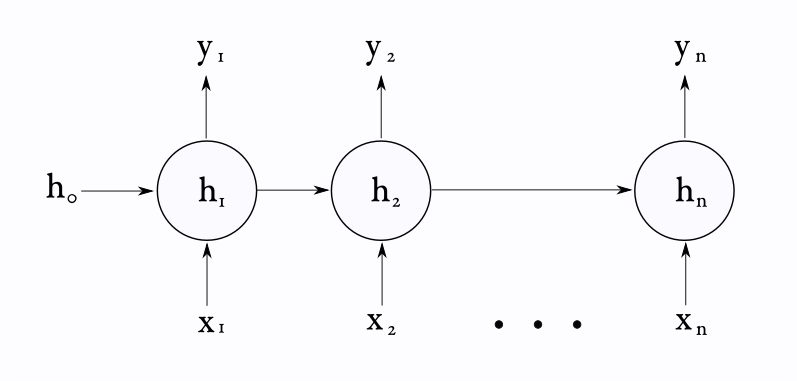
\includegraphics[width=0.5\textwidth]{pics/rnn_network}
  \caption{RNN for NER}
  \label{fig:rnn_network}
\end{figure}

Recurrent neural networks (RNN) have been succesfully employed on numerous NLP tasks such as
language modelling, POS tagging, speech recognition and NER. Different from feedforward neural networks, 
RNNs can retain information in their internal state, making them more suitable for processing sequences, 
and consequently for solving text related tasks. In NER, the network outputs one label for each input 
vector as showed in Figure \ref{fig:rnn_network}. 

Although RNNs are theoretically capable of learning long term dependencies, in practice 
it might be difficult. Long short term memory networks (LSTM) were introduced by Hochreiter 
and Schmidhuber \cite{Hochreiter1997} with this problem in mind and have been 
popularized since them. LSTM cell implementations vary slightly in the literature.
Our implementation has the following definition:

\begin{flalign*}
\Gamma_i^{<t>} &= \sigma(W_i[x^{<t>},h^{<t-1>}] + b_i) &\\
\Gamma_f^{<t>} &= \sigma(W_f[x^{<t>},h^{<t-1>}] + b_f) &\\ 
c^{<t>}        &= \Gamma_f^{<t>} \circ c^{<t-1>} + \Gamma_i^{<t>} tanh(W_c[x^{<t>},h^{<t-1>}] + b_c) &\\
\Gamma_o^{<t>} &= \sigma(W_o[x^{<t>},h^{<t-1>}] + b_o) &\\
h^{<t>}        &= \Gamma_o^{<t>} \circ tanh(c^{t}) &
\end{flalign*}

\begin{figure}
  \centering
  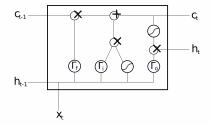
\includegraphics[width=0.5\textwidth]{pics/lstm_cell}
  \caption{LSTM Cell}
  \label{fig:lstm_cell}
\end{figure}

where $ \sigma $ is the logistic sigmoid function. $ \Gamma_i $, $ \Gamma_f $, and $ \Gamma_o $ are the input,
forget and output gates, respectively. And $ W $ with a subscript is the weight 
matrix corresponding to that gate. Variable $ c^{<t>} $ is the cell 
state and $ h^{<t>} $ is the hidden state, with the vector $ [x^{<t>},h^{<t-1>}] $ 
being formed by concatenating the current input vector $ x^{<t>} $ and the hidden vector 
from the previous timestep $ h^{<t-1>} $. A visual description of our LSTM cell is 
provided in figure \ref{fig:lstm_cell}.
This implementation differs from the LSTM cell described in Huang et al. \cite{Huang2015}
in that the input gate $ \Gamma_i $ and the forget gate $ \Gamma_f $
do not take input from the previous cell state $ c^{<t-1>} $ and the output gate does
not take input from the current cell state $ c^{<t>} $. The cell state and the control gates 
are what makes the LSTM cell better at modelling long term dependencies in comparison
to a regular RNN.

In NER related tasks, both past and future words are important when deciding the
label at time $ t $, but a regular LSTM network only takes past features in consideration. 
A bidirectional LSTM solves this problem by stacking two regular LSTMs, and feeding
them with observations in opposite directions. The first LSTM receives the forward
states and the second LSTM receives the backward states. The hidden states from both 
networks can be concatenated at each time step to produce the output label. With this 
architecture, Bidirectional LSTMs have information from all input features in the sequence at 
any given timestep.

\subsubsection{LSTM-CRF}
\label{sssec:lstm_crf}

\begin{figure}
  \centering
  \includegraphics[width=0.5\textwidth]{pics/bi_lstm_crf}
  \caption{Bidirectional LSTM-CRF}
  \label{fig:bi_lstm_crf}
\end{figure}

Huang et al. \cite{Huang2015} proposed a bidirectional LSTM with a CRF layer (LSTM-CRF) on the output to tackle
the sequence tagging problem. The CRF layer jointly decodes labels for the whole sentence instead
of predicting each label individually. This architecture achieved an F1 score of 90.10 on the English
data from CONLL-2003 shared task \cite{Sang2003}, in contrast to 85.17 for a bidirectional LSTM without the CRF layer. 
In our experiments, the LSTM-CRF architecture used a bidirectional LSTM with 100 
hidden states, no peepholes and an input and output dropout layers with a dropout
rate of 0.5. The dropout layers have proven to be very important to prevent overfitting 
and allow better generalization.

\subsubsection{LSTM-CRF + CNN character representations}
\ref{sssec:lstm_crf_cnn}

\begin{figure}
  \centering
  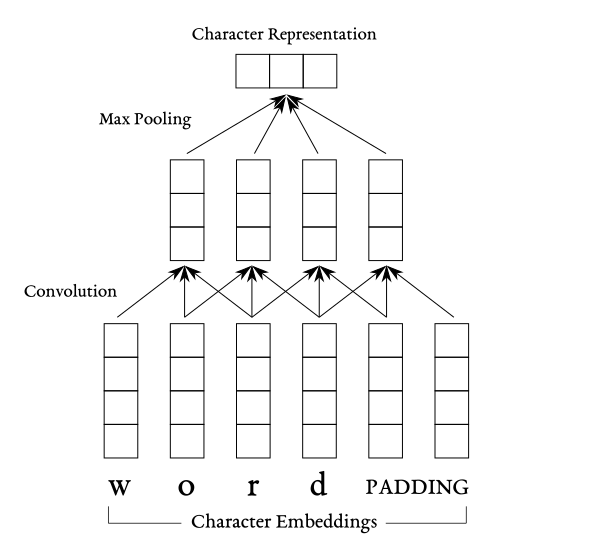
\includegraphics[width=0.5\textwidth]{pics/cnn}
  \caption{CNN}
  \label{fig:cnn}
\end{figure}

Ma and Hovy \cite{Ma2016} proposed adding a convolutional neural network (CNN) layer 
on top of a bidirectional LSTM-CRF to encode character-level information. The CNN
layer is described visually in Figure \ref{fig:cnn}, it receives
only character embeddings as inputs. The character representations generated by the CNN 
are combined with word level representations and then fed to the Bidirectional LSTM with
a CRF output layer described in section \ref{sssec:lstm_crf}.
This architecture can learn morphological features that are very
useful in the NER task, since similar named entities often present morphological similarities. 
This architecture obtained an F1 score of 91.21 in the ConLL2003 dataset. In our experiments, 
the LSTM-CRF architecture with CNN character representations uses a one dimensional convolutional 
neural network with 30 filters and a window size of three characters on top of the LSTM-CRF architecture.
The character embeddings fed to the CNN had 30 dimensions that were randomly initialized.

\subsubsection{LSTM-CRF + LSTM character representations}

\begin{figure}
  \centering
  \includegraphics[width=0.5\textwidth]{pics/lstm_char_representations}
  \caption{LSTM character representations}
  \label{fig:lstm_char}
\end{figure}

Lample et al \cite{Lample2016} suggested using an a bidirectional LSTM to model character-level 
representations on a bidirectional LSTM-CRF. Combining both the forward and backward 
LSTM representations to form the character representation, as described in figure \ref{fig:lstm_char}. 
This character representation is also combined with a word representation and fed to a LSTM-CRF network. 
The forward LSTM is expected to be a better
representation of the suffix of a token, and the backward LSTM is expected to be a
better representation of the prefix of a token. This differentiates the architecture
from the CNN based approach described in Section \ref{sssec:lstm_crf_cnn}, because CNN filters 
discover positional invariant features, while LSTMs can better represent suffixes and prefixes. In our experiments, 
the LSTM-CRF architecture with LSTM character representations was implemented with a bidirectional LSTM
with 25 hidden states, producing character representations of size 50. The character embeddings
had 30 dimensions that were randomly initialized.

\subsubsection{Network training}

The neural models were trained with mini batch Stochastic Gradient Descent over 50 epochs with batch size 10,
learning rate 0.01, momentum 0.9 and decay rate 0.05. We used early stopping \cite{Caruana2000} to select the best 
parameters, considering the F1 measure in the validation set. All neural models used 
GloVe 100-dimensional word embeddings \cite{Pennington2014} that were fine tuned during training,
they have a vocabulary size of 400.000 words.
In the case of NER on HTML, word embeddings work similar to a gazetteer. Named entities 
of a same type have similar embeddings, so good word embeddings can achieve exceptional 
performance with little training and without a gazetteer. 

\section{NER on HTML Dataset}

We constructed a novel dataset to evaluate the performance of multiple NER models
at the web information extraction task. The task consists of finding researcher
names in faculty listings from multiple web pages. This would be the 
first step in linking researcher profiles from university websites to their entries
in public databases such as DBLP \footnote{http://dblp.uni-trier.de/}. Unlike many
information extraction datasets, each web page in the dataset comes from a different 
website, and therefore has a different format, what makes many information
extraction approaches impractical. The idea is to explore systems that are general 
enough to allow efficient name extraction from many different sources while requiring
no supervision between different websites. 

This task would be similar to the task of labeling authors in comments
However, we wanted to evaluate models without relying on any sophisticated data record
segmentation system. In many cases, entity annotation may precede the segmentation
phase in web data extraction methods, so annotators have to be able to work with
raw HTML data. Because of the type of documents present in the dataset, many sentences 
contained only one or two tokens, while other documents contained long texts.
Finally, all tokens were tagged using the IOB scheme put forward by
Ramshaw and Marcus \cite{Ramshaw1995}. 

\subsection{Data}

\begin{table}[h]
  \small
  \begin{center}
    \begin{tabular}{ |l|l|l|l|l| }
      \hline
      Data file & Documents & Sentences & Tokens & Names \\
      \hline
      Training    & 92 & 28958 & 124984 & 6382 \\
      Validation  & 28 & 9117  & 39748  & 2258 \\
      Test        & 25 & 5790  & 26995  & 1949 \\
      \hline
    \end{tabular}
  \end{center}
  \caption{Number of HTML pages, sentences and tokens in each data file}
  \label{tab:dataset}
\end{table}

The dataset was divided in a training, validation and test set. Table \ref{tab:dataset} contains
a description of the data files. The validation set was used in the early stopping validation strategy
on neural model and CRF training, while results were evaluated by comparing results in the test set.

\subsection{Features}

Twelve categorical features were also present with each token in the dataset. They 
are presented in table \ref{tab:features}.

\begin{table}[h]
  \small
  \begin{center}
    \begin{tabular}{ |l|l| }
      \hline
      Feature & Description \\
      \hline
      1  & Unaccented lowercase token \\
      2  & Exact gazetteer match \\
      3  & Partial gazetteer match \\
      4  & Log name gazetteer count\\
      5  & Log word gazetteer count\\
      6  & Email \\
      7  & Number \\
      8  & Honorific \\
      9  & URL \\
      10 & Is capitalized \\
      11 & Is a punctuation sign \\
      12 & HTML tag + parent \\
      13 & CSS class \\
      \hline
    \end{tabular}
  \end{center}
  \caption{Features present in the bla dataset}
  \label{tab:features}
\end{table}

The unaccented lowercase token was used as the key for the Glove-100 embedding lookup.
A gazetteer was constructed from a researcher list extracted from DBLP with 1.595.771
names. Feature 2 represents an exact match of a sequence of tokens to any of the 1.595.771 
names, and feature 3 represents a partial match. Feature 4 is the rounded logarithm of 
the frequency of a token in the gazetteer, and feature 5 is the rounded logarithm of the frequency
of a token in a word corpus obtained through a random crawl in university websites.
Features 6 to 11 represent a simple regular expression match to an email, number, 
honorific, URL, capitalization and punctuation sign.

Feature 12 represents the HTML enclosing tag and its parent concatenated. Feature 13
represents all CSS classes concatenated. These features are not very useful in a general
sense, because every HTML document has a different format, so only because a named entity
occurs inside a given HTML tag in a document we cannot say it is more likely to be the case 
in other documents. However, these features can be trained with the self-training strategy 
for HMMs described in section \ref{sssec:self_training}. In all other models these features 
were ignored.

\section{Experiments}

We conducted two experiments to evaluate the best models for named entity recognition
on HTML in the context of web data extraction. In the first experiment, we used the
whole training set (90 documents). In the second experiment, the training set was split 
into five non overlapping sets with only 18 documents, but the test set was kept unchanged. 
The goal of this second experiment 
was to evaluate models when training data is scarce, since labelling data can be a very 
time consuming task.

Evaluation of model performance in this task was measured with the precision, recall and 
F1 scores (Van Rijsbergen, 1975). Precision is the percentage of named entities found by 
the model that are correct. Recall is the percentage of named entities that are present
in the corpus and were found by the model. The F1 score is a composite measure that combines
precision and recall with the formula:

\begin{equation}
F1 = \frac{2 * precision * recall}{precision + recall}
\end{equation}

\begin{table}[h]
  \small
  \begin{center}
    \begin{tabular}{ |l|l| }
      \hline
      Model & Description \\
      \hline
      hmm-1         & Regular HMM \\
      hmm-2         & HMM with $ k=2 $ \\
      hmm-3         & HMM with $ k=3 $ \\
      crf           & Linear chain conditional random fields \\
      lstm-crf      & LSTM-CRF model \cite{Huang2015} \\
      lstm-crf-cnn  & LSTM-CRF with CNN character representations \cite{Ma2016} \\
      lstm-crf-lstm & LSTM-CRF with LSTM character representations \cite{Lample2016} \\
      \hline
    \end{tabular}
  \end{center}
  \caption{Model descriptions}
  \label{tab:models}
\end{table}

Named entities were only considered to be correct if they were a complete match of the 
corresponding entity in the dataset. The models evaluated are presented in Table \ref{tab:models}.
We evaluated the models using the complete set of features, presented in 
table \ref{tab:features} and no features besides word embeddings for neural models and
CRFs, and unaccented words for HMMs. To represent models with the complete set of features
we added a "+F" suffix to the model name. Additionally, HMMs were evaluated with and
without the self training strategy. To represent HMMs that use the self training strategy
we added the suffix "+ST" to the model name.
Results were reported for the validation and test sets in experiment 1 and only for the
test set in experiment 2. In the second experiment, precision, recall and F1 scores were 
averaged over the five runs. The standard deviation is presented next to the measures.

\subsection{Experiment 1: complete dataset}

\begin{table}[h]
  \small
  \begin{center}
    \begin{tabular}{ |l|l|l|l|l|l|l| }
      \hline
      \multirow{2}{*}{Model} & \multicolumn{3}{c|}{Validation} & \multicolumn{3}{c|}{Test} \\
                             & \multicolumn{1}{c}{Precision} & \multicolumn{1}{c}{Recall} & \multicolumn{1}{c|}{F1}
                             & \multicolumn{1}{c}{Precision} & \multicolumn{1}{c}{Recall} & \multicolumn{1}{c|}{F1} \\
      \hline
      hmm-1	      & 0.6965 & 0.5749 & 0.6299 & 0.6263 & 0.4431 & 0.5190 \\
      hmm-2	      & 0.7047 & 0.6286 & 0.6645 & 0.6480 & 0.5222 & 0.5783 \\
      hmm-3	      & 0.6127 & 0.6141 & 0.6134 & 0.5471 & 0.4634 & 0.5018 \\
      crf	      & 0.7237 & 0.6650 & 0.6931 & 0.6734 & 0.5879 & 0.6278 \\
      lstm-crf        & 0.8607 & 0.8848 & 0.8726 & 0.8546 & 0.8294 & 0.8418 \\
      lstm-crf-cnn    & 0.9221 & 0.9206 & 0.9214 & 0.9030 & 0.8283 & 0.8640 \\
      lstm-crf-lstm   & 0.9129 & 0.9441 & 0.9282 & 0.8906 & 0.8807 & 0.8856 \\
      \hline
    \end{tabular}
  \end{center}
  \caption{Precision, recall and F1 in the complete dataset}
  \label{tab:experiment1}
\end{table}

Experiment 1 consists of testing the models on the complete NER on HTML dataset 
described in section \ref{sec:ner_dataset}. Table \ref{tab:experiment1} shows the 
results for models that employed no features, except for the words in the text
in the case of HMMs and Glove-100 word embeddings in the case of CRFs and Neural Models.
Without carefully designed features and a gazetteer, HMMs and CRFs have a very 
poor performance, achieving only 57.83 for HMM-2 and 62.78 for CRF in the test set. 
The neural models however achieved high F-scores, even with no features. The
plain LSTM-CRF architecture improved significantly in comparison to the conventional CRF,
and the LSTM-CRF architectures with neural character representations boosted the F1 score
by 2.32 for CNN representations and 4.38 for LSTM representations, showing that they are 
able to learn morphological features automatically, and that at least in the NER tasks LSTM 
character representations are superior, perhaps because they are able to differentiate 
suffixes and prefixes, while CNNs are position invariant. This experiment also shows that
pretrained word embeddings can be used to identify named entities in HTML, where
textual context is very limited without resorting to gazetteers.

\begin{table}[h]
  \small
  \begin{center}
    \begin{tabular}{ |l|l|l|l|l|l|l| }
      \hline
      \multirow{2}{*}{Model} & \multicolumn{3}{c|}{Validation} & \multicolumn{3}{c|}{Test} \\
                             & \multicolumn{1}{c}{Precision} & \multicolumn{1}{c}{Recall} & \multicolumn{1}{c|}{F1}
                             & \multicolumn{1}{c}{Precision} & \multicolumn{1}{c}{Recall} & \multicolumn{1}{c|}{F1} \\
      \hline
      hmm-1+F	      & 0.6061 & 0.7282 & 0.6616 & 0.7106 & 0.7633 & 0.7360 \\
      hmm-2+F	      & 0.6279 & 0.7550 & 0.6856 & 0.7521 & 0.7810 & 0.7663 \\
      hmm-3+F	      & 0.6573 & 0.7819 & 0.7142 & 0.7523 & 0.7795 & 0.7657 \\
      hmm-1+F+ST      & 0.7032 & 0.9077 & 0.7925 & 0.7522 & 0.8663 & 0.8052 \\
      hmm-2+F+ST      & 0.7321 & 0.9172 & 0.8143 & 0.7737 & 0.8789 & 0.8230 \\
      hmm-3+F+ST      & 0.7551 & 0.9172 & 0.8283 & 0.7961 & 0.8534 & 0.8237 \\
      crf+F	      & 0.8982 & 0.9128 & 0.9054 & 0.8812 & 0.8298 & 0.8547 \\
      lstm-crf+F      & 0.9378 & 0.9441 & 0.9409 & 0.8959 & 0.8807 & 0.8883 \\
      lstm-crf-cnn+F  & 0.8998 & 0.9799 & 0.9382 & 0.8910 & 0.9295 & 0.9098 \\
      lstm-crf-lstm+F & 0.9495 & 0.9569 & 0.9532 & 0.9163 & 0.8888 & 0.9023 \\
      \hline
    \end{tabular}
  \end{center}
  \caption{Precision, recall and F1 in the complete dataset}
  \label{tab:experiment1f}
\end{table}

Table \ref{tab:experiment1f} shows the results on experiment 1 for models
that employed all features described on Table \ref{tab:features}. In this case
we see that conventional models like HMMs, and CRFs can become competitive with
the right selection of features and a good gazetteer, however they still lose
to the best neural model without features showing their limitation. We can also
see that the self training strategy for HMMs improved the quality of the results
significantly on all cases, boosting both precision and recall.

The neural models also improved a little with the addition of features. The fact that 
the LSTM-CRF gets much closer to the neural models with character representations
shows that the LSTM and CNN character representations were probably able to learn 
at least part of the features automatically, and when we add them explicitly,
the difference in performance becomes less noticeable.

\subsection{Experiment 2: reduced dataset}

\begin{table}[h]
  \small
  \begin{center}
    \begin{tabular}{ |l|l|l|l|}
      \hline
      \multirow{2}{*}{Model} & \multicolumn{3}{c|}{Test} \\
                             & \multicolumn{1}{c}{Precision} & \multicolumn{1}{c}{Recall} & \multicolumn{1}{c|}{F1} \\
      \hline
      hmm-1           & 0.5333 (0.111) & 0.8409 (0.111) & 0.6527 (0.111) \\
      hmm-2           & 0.5333 (0.111) & 0.8409 (0.111) & 0.6527 (0.111) \\
      hmm-3           & 0.5333 (0.111) & 0.8409 (0.111) & 0.6527 (0.111) \\
      crf             & 0.5333 (0.111) & 0.8409 (0.111) & 0.6527 (0.111) \\
      lstm-crf        & 0.5333 (0.111) & 0.8409 (0.111) & 0.6527 (0.111) \\
      lstm-crf-cnn    & 0.5333 (0.111) & 0.8409 (0.111) & 0.6527 (0.111) \\
      lstm-crf-lstm   & 0.5333 (0.111) & 0.8409 (0.111) & 0.6527 (0.111) \\
      \hline
    \end{tabular}
  \end{center}
  \caption{Precision, recall and F1 in the small dataset}
  \label{tab:experiment2}
\end{table}

The second experiment aimed at evaluating the performance of sequence models
when the dataset is reduced to only 18 labeled documents. A feasible amount of 
labelling in most WDE tasks. The experiment was repeated in five non overlapping 
sets of training data, and the results were averaged. Table \ref{tab:experiment2} 
describes the results for models without any features. We only present results
for the test set in this experiment. The standard deviation is shown next to each
measure.

We can see that the performance of all models was reduced in comparison 
to experiment 1. That is to be expected.

\begin{table}[h]
  \small
  \begin{center}
    \begin{tabular}{ |l|l|l|l|}
      \hline
      \multirow{2}{*}{Model} & \multicolumn{3}{c|}{Test} \\
                             & \multicolumn{1}{c}{Precision} & \multicolumn{1}{c}{Recall} & \multicolumn{1}{c|}{F1} \\
      \hline
      hmm-1+F         & 0.5333 (0.111) & 0.8409 (0.111) & 0.6527 (0.111) \\
      hmm-2+F         & 0.5333 (0.111) & 0.8409 (0.111) & 0.6527 (0.111) \\
      hmm-3+F         & 0.5333 (0.111) & 0.8409 (0.111) & 0.6527 (0.111) \\
      hmm-1+F+ST        & 0.5333 (0.111) & 0.8409 (0.111) & 0.6527 (0.111) \\
      hmm-2+F+ST        & 0.5333 (0.111) & 0.8409 (0.111) & 0.6527 (0.111) \\
      hmm-3+F+ST        & 0.5333 (0.111) & 0.8409 (0.111) & 0.6527 (0.111) \\
      crf+F           & 0.5333 (0.111) & 0.8409 (0.111) & 0.6527 (0.111) \\
      lstm-crf+F      & 0.5333 (0.111) & 0.8409 (0.111) & 0.6527 (0.111) \\
      lstm-crf-cnn+F  & 0.5333 (0.111) & 0.8409 (0.111) & 0.6527 (0.111) \\
      lstm-crf-lstm+F & 0.5333 (0.111) & 0.8409 (0.111) & 0.6527 (0.111) \\
      \hline
    \end{tabular}
  \end{center}
  \caption{Precision, recall and F1 in the small dataset}
  \label{tab:experiment2f}
\end{table}

We can see that the performance of all models was reduced in comparison 
to experiment 1. That is to be expected.

\section{Conclusion}

Deep learning models are better blabla.

HMMs are competitive but demand feature engineering blabla.

Token morphology is necessary.

Label dependency is necessary.
Our name extraction method achieved 94.40\% precision, 97.61\% recall 
and 0.9597 F-measure on a corpus of 152 faculty directory web pages from
49 different countries with 11782 researcher names. 
The model is tuned for the particular problem of name extraction, 
but we believe this result can be generalized to solve other data extraction 

\end{document}
